\chapter{Implementation}

We decided to implement the last paper to compute Wasserstein distances on images in a efficient way. We then use convolutional Sinkhorn in SVM as Marco Cuturi used Sinkhorn in his paper to classify images of the MNIST digit database \cite{Cut}. The implementation of the convolutional Wassertein distance has been written in C++. We then write the Gramm matrix of a subset of the MNIST database in a file and use it in a Python script to use SVM from Sklearn library.

\paragraph{How to use our code}
OpenMP has been used to parallelize the code. If you don't have OpenMP already install, you can install it with \verb|sudo apt install libomp-dev|.
To compile the C++ code you just have to type \verb|make|. Then you need to obtain the train image datatset and the train label dataset of the MNIST database \url{http://yann.lecun.com/exdb/mnist/}. To do so you have to run the script \verb|get_mnist.sh| which will download and rename the files correctly. The executable \verb|main| created by \verb|make| command can be used in four ways.
\begin{itemize}
	\item  \verb|./main bar| to reproduce an image similar to the \figurename~\ref{barp}; An image containing different barycenters of four shapes.
	\item \verb|./main card| to reproduce images similar to the \figurename~\ref{cardp}; An interpolation of two images of cards.
	\item \verb|./main wass > kernel.txt| to compute a kernel with the convolutional Wasserstein distance of \verb|N_TRAIN| images of the MNIST dataset. We project \verb|N_TEST| other digit images of the MNIST dataset on the kernel space created. You can change the parameter \verb|N_TRAIN| and \verb|N_TEST| at the beginning of the file \verb|src/main.cpp|. The kernel will then be written if the file \verb|kernel.txt|.
	\item \verb|./main eucl > kernel.txt| to do the same as the previous command but with Euclidean distance instead of Wasserstein distance. 
\end{itemize}
Finally when a kernel file is computed you can test SVM on it thanks to the python script \verb|learning.py|. Because computing Wasserstein kernel may take a while we provide the Wasserstein kernel \verb|kernels/wass.txt| and the Euclidean kernel \verb|kernels/eucl.txt|. You can then run:
\begin{center}
	\verb=python3 learning.py < [kernels/wass.txt | kernels/eucl.txt]=
\end{center}
It will print the performances of these two kernels, show the projection of the data on the two principle components and finally show the kernel matrix.

\paragraph{Barycenters}
We first computed some barycenters to be sure that everything works. The code for computing Wasserstein distances and barycenters is in the file \verb|src/wasserstein.cpp|. The code that produce the barycenters that we will present is in the file \verb|examples.cpp|. The first example is the reproduction of \figurename~\ref{barp}. Here is what we obtained:

\begin{figure}[h]
	\centering
	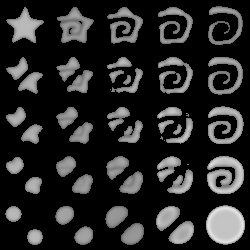
\includegraphics[scale=0.5]{bars_own.png}
	\caption{Reproduction of \figurename~\ref{barp}}
\end{figure}

The result seems to be correct. We then try on larger images, the card images that we can find in the original paper presenting convolutional Wassertein \cite{Goe++}. Here is what we obtained:

\begin{figure}[h]
	\centering
	\begin{tikzpicture}
		\node[] at (0, 0) {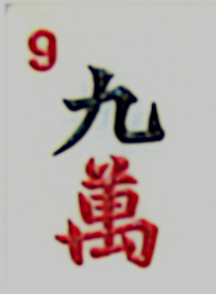
\includegraphics[scale=0.3]{bar0.png}};
		\node[] at (2.8, 0) {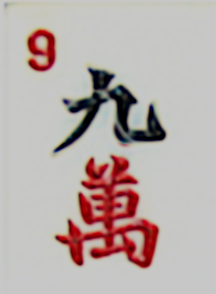
\includegraphics[scale=0.3]{bar3.png}};
		\node[] at (5.6, 0) {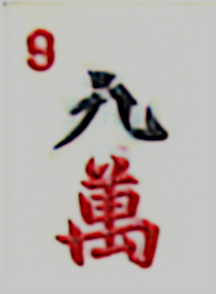
\includegraphics[scale=0.3]{bar6.png}};
		\node[] at (8.4, 0) {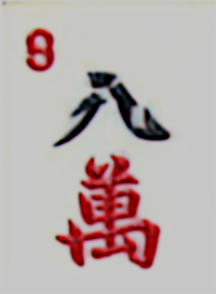
\includegraphics[scale=0.3]{bar8.png}};
		\node[] at (11.2, 0) {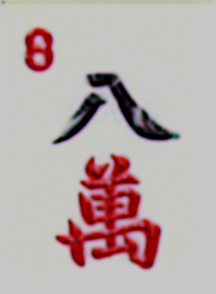
\includegraphics[scale=0.3]{bar11.png}};
		\node[] at (14, 0) {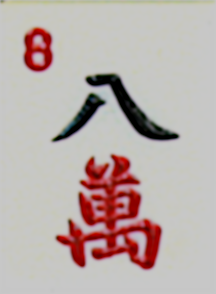
\includegraphics[scale=0.3]{bar14.png}};
	\end{tikzpicture}
	\caption{Reproduction of \figurename~\ref{cardp}}
\end{figure}

\paragraph{SVM usage}
As proposed in the paper of Cuturi \cite{Cut}, we used the Wasserstein distance to compute the Gram matrix for 500 image and we used it as a kernel in a SVM. On a test set of 1500 images we obtained 92.4\% of good answers. Whereas with a kernel using Euclidean distance we obtain a good answer on only 88.4\%. To check these results you can run the python script \verb|learning.py| on the two kernels that are in the \verb|kernels| folder.